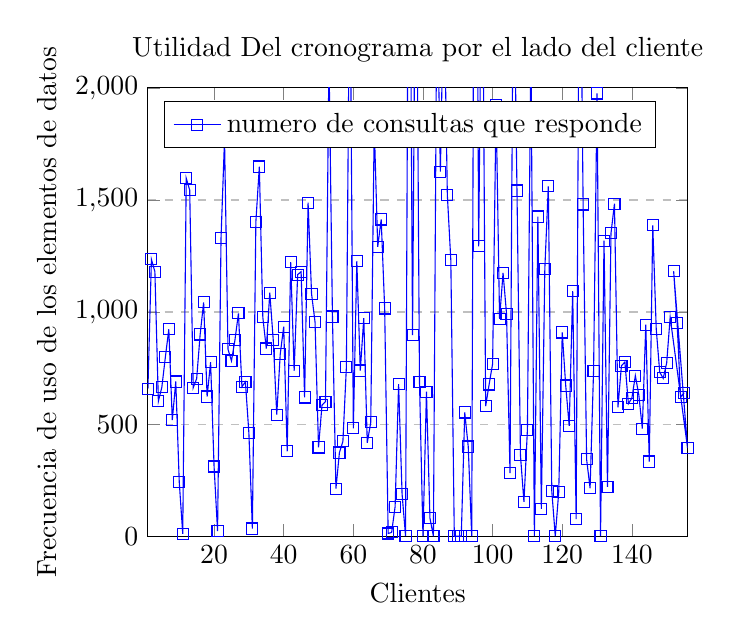
\begin{tikzpicture}
\begin{axis}[
    title={Utilidad Del cronograma por el lado del cliente},
    xlabel={Clientes},
    ylabel={Frecuencia de uso de los elementos de datos},
    xmin=1, xmax=156,
    ymin=0, ymax=2000,
    xtick={},
    ytick={},
    legend pos=north west,
    ymajorgrids=true,
    grid style=dashed,
]

\addplot[
    color=blue,
    mark=square,
    ]
    coordinates {
    %USO EXACTO
    (1,658)
(2,1235)
(3,1180)
(4,602)
(5,665)
(6,798)
(7,923)
(8,518)
(9,690)
(10,241)
(11,10)
(12,1597)
(13,1544)
(14,662)
(15,703)
(16,900)
(17,1043)
(18,623)
(19,776)
(20,311)
(21,23)
(22,1331)
(23,1771)
(24,834)
(25,782)
(26,876)
(27,994)
(28,667)
(29,688)
(30,460)
(31,34)
(32,1402)
(33,1649)
(34,977)
(35,837)
(36,1086)
(37,874)
(38,542)
(39,812)
(40,935)
(41,379)
(42,1223)
(43,738)
(44,1167)
(45,1180)
(46,619)
(47,1488)
(48,1081)
(49,955)
(50,396)
(51,585)
(52,600)
(53,2140)
(54,980)
(55,212)
(56,373)
(57,423)
(58,754)
(59,2686)
(60,481)
(61,1227)
(62,739)
(63,973)
(64,417)
(65,508)
(66,1834)
(67,1291)
(68,1413)
(69,1016)
(70,12)
(71,17)
(72,132)
(73,678)
(74,188)
(75,0)
(76,3581)
(77,897)
(78,3082)
(79,689)
(80,0)
(81,645)
(82,81)
(83,0)
(84,2487)
(85,1626)
(86,2493)
(87,1522)
(88,1231)
(89,0)
(90,0)
(91,0)
(92,552)
(93,400)
(94,0)
(95,4394)
(96,1293)
(97,2936)
(98,580)
(99,677)
(100,769)
(101,1925)
(102,970)
(103,1174)
(104,993)
(105,281)
(106,2710)
(107,1542)
(108,361)
(109,153)
(110,475)
(111,2197)
(112,0)
(113,1426)
(114,122)
(115,1193)
(116,1561)
(117,202)
(118,0)
(119,198)
(120,909)
(121,672)
(122,492)
(123,1093)
(124,76)
(125,3024)
(126,1480)
(127,343)
(128,214)
(129,738)
(130,1975)
(131,0)
(132,1318)
(133,220)
(134,1351)
(135,1483)
(136,575)
(137,760)
(138,777)
(139,591)
(140,616)
(141,716)
(142,630)
(143,480)
(144,944)
(145,333)
(146,1387)
(147,924)
(148,732)
(149,704)
(150,773)
(151,977)(156,393)
(152,1182)
(153,950)
(154,620)
(155,640)

    };
    \legend{numero de consultas que responde}

\end{axis}
\end{tikzpicture}

